\chapter{Marco Teórico}

 En este capitulo se aborda el marco teórico necesario para comprender más fácilmente el desarrollo de los capítulos posteriores. Se analiza el problema del tráfico en general y como se buscan soluciones como por ejemplo con la construcción de Corredores exclusivos para el transporte publico. En este contexto se detalla el Corredor de Garzón tanto su descripción como sus problemas. Luego se da un breve repaso sobre los simuladores de trafico y la teoría detrás de los algoritmos evolutivos. Para finalizar se encuentra una lista con trabajos relacionados para mostrar otras variantes y opciones.

\section{Problema del tránsito vehicular}

En gran parte del mundo se está produciendo un crecimiento sostenido del parque automotor lo que ocasiona una serie de problemas que afectan la calidad de vida de las personas relacionados con el agravamiento de las congestiones vehiculares \citep{Cepal2003}.

Este problema tiene un gran impacto en el desarrollo de las ciudades por lo que es un componente principal en los planes estratégicos para su crecimiento.

La congestión ocasiona una progresiva merma en la velocidad promedio de circulación, lo que incrementa la duración de los viajes, aumenta el consumo de combustible y la contaminación atmosférica y sonora, lo que repercute directamente en la salud de las personas. 
además se genera una exigencia en las vías de tránsito que ocasiona un deterioro mayor de calles y rutas.

Uruguay no escapa a este fenómeno en particular Montevideo, donde el aumento del parque automotor está en ascenso constante desde el 2005 \citep{INE2014} 
Y según proyecciones el crecimiento seguiría en un promedio de 4.5\% anual hasta el 2020. \citep{BBVA2013}

Esto viene de la mano con el sostenido aumento de las ventas de vehículos  desde el 2003 \citep{Autoanuario2014}

Los expertos indican que la congestión ya está instalada y la infraestructura vial no acompasó este crecimiento. además se indica que Montevideo es la ciudad con más semáforos por automóvil en Latinoamérica. Con más de 620 cruces semaforizados, alguno de los cuales no están coordinados.\citep{Subrayado2013}

El crecimiento en la circulación de automóviles provoca que baje el nivel de aceptación del transporte publico cuyo servicio en general es ineficiente. Para resolver este problema las autoridades suelen optar por sistemas de transporte costosos como los Metros pero se ha demostrado que existen otras opciones viables como el BRT (Bus Rapid Transit / ómnibus de transito rápido).\citep{BRT_Dial} 

En el caso de Montevideo para solucionar este problema se esta implementando el plan de movilidad urbana \citep{PlanMovilidad} con el objetivo de mejorar la eficiencia del transporte publico y democratizar el acceso al mismo. El sistema de transporte esta inspirado en un BRT con la construcción de varios corredores exclusivos en la ciudad. En la siguiente sección se dará mas información sobre los BRT, corredores urbanos y en particular el Corredor de Garzón.



\section{Corredores Urbanos de trafico}

El corredor urbano de trafico o también llamado corredor segregado se caracteriza por una separación física entre el carril de circulación de los autobuses y los carriles para el resto del tráfico y esta es la principal diferencia con un concepto similar llamado "carril de solo bus". Los carriles de solo bus se separan por líneas horizontales que son pintadas en la calle indicando que solo pueden circular autobuses por ese medio y los corredores segregados una separación en cemento que imposibilita el cambio de carriles. Los carriles de solo bus suelen fracasar por falta de control que evite que el tráfico los invada. En el caso de Montevideo mas allá de ser muy difícil de controlar que no se invada el carril, al hacer los carriles de solo bus sobre la derecha, es necesario que el transporte privado invada el carril al doblar a la derecha y que taxis lo invadan para levantar pasajeros por estar al lado de la vereda.  

Los corredores segregados a nivel (sin hacer viaductos) cruzan las intersecciones mediante semáforos, lo que puede reducir mucho la capacidad del sistema. Las corredores segregados a distinto nivel evitan esos conflictos al construirse de forma que los carriles del autobús quedan completamente separados del resto del tráfico. 

Las ciudades de países en vías de desarrollo deben estudiar si pueden instalar corredores pues son fundamentales para conseguir mayores velocidades en el sistema. Pero hay muchas posibilidades y no todas pueden ser aplicables por el contexto zonal, cultural o de inversión necesaria. Para intentar catalogar todos los corredores existentes, para poder saber que tan bueno puede llegar a ser un corredor en la fase de estudio del problema, la CUTR (Center for Urban Transportation Research) crea el National BRT Institute con la consigna de facilitar el intercambio de conocimientos y la innovación para aumentar la velocidad, la eficiencia y confiabilidad del servicio de autobuses. Se generan buenas practicas, se presentan estudios realizados en distintas zonas antes y despues de implementados los corredores, y se crea un standard que califica que tan bueno es un corredor BRT.
http://www.cutr.usf.edu/programs-1/national-bus-rapid-transit-institute/

Bus Rapid Transit (BRT) es una solución innovadora, de alta capacidad y de menor costo para el transporte público que puede alcanzar el rendimiento y los beneficios de modos ferroviarios con un costo significativamente menor. Se trata de un sistema integrado de transporte basado en autobuses para el transporte de los pasajeros a sus destinos de manera rápida y eficiente. Al mismo tiempo ofrece la flexibilidad necesaria para satisfacer una variedad de condiciones locales. Los elementos del sistema de BRT pueden ser fácilmente personalizados a las necesidades de la comunidad e incorporan tecnologías de última generación de bajo costo que atraen a más pasajeros y en última instancia ayudan a reducir la congestión de tráfico en general.

Un BRT contiene características similares a un tren ligero o el sistema de metro por ese motivo es mucho más confiable, conveniente y más rápido que los servicios regulares de autobús. Con las características adecuadas, el BRT es capaz de evitar las causas de los retrasos que suelen tener los servicios regulares de autobús, como estar atrapado en el tráfico y hacer cola para pagar a bordo.

\begin{figure}[h]
	\centering
	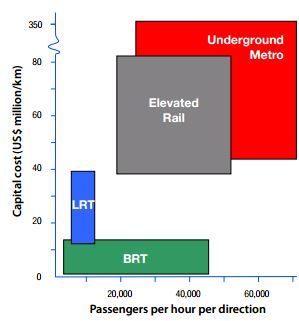
\includegraphics[width=0.7\linewidth]{Figures/costo_transporte}
	\caption{Gráfica de costos de transporte en función de la gente transportada, BRT (Bus Rapid Transit), LRT(Light Rail Train)- Imagen original extraída de \citep{ITDP}		
	}
	\label{fig:Grafica de costos de otros medios de transporte}
\end{figure}
	
\subsection{Corredor de Garzón}	

COMPLETAR
Estas referencias son las que usamos en el paper:
\citep{olivera2013}
\citep{olivera2015}	


Esta localizado al Nordeste de Montevideo Uruguay, fue construido como parte de un plan de movilidad que incluye otros 4 corredores de la ciudad. Tomando en cuenta de un extremo al otro conecta Colon con Paso Molino y teniendo 6.5km de largo, atraviesa muchas calles importantes como Millan p.e. que lleva a una autopista (Ruta 5). Es importante aclarar que no es solo una conexión de extremo a extremo ya que barrios como Sayago y otros constan de una gran cantidad de habitantes.
Consiste básicamente en 3 calles paralelas e independientes; donde 2 de ellas son de dos carriles de una sola mano y entre medio de estas esta una calle doble vía con un carril para cada vía que es exclusivamente usado por ómnibus.


Se considera un BRT por motivos destacar puntos acumulados:

Recomendaciones del standard no aplicadas totalmente al corredor:
\begin{itemize}
	\item SEMÁFOROS. Un corredor debe de funcionar al igual que una autopista en el sentido de que una vez que se entra debería ser posible mantener la velocidad máxima sin tener que parar seguido por lo que no deberían de haber semáforos cerca uno del otro, de haberlos la sincronización será la clave para minimizar los tiempos de espera.
	\item CALLES PARALELAS. Tener calles paralelas es de vital importancia para un corredor ya que una de las formas de minimizar los tiempos de espera es prohibir los giros a la izquierda, y una calle paralela provee la facilidad de poder realizarlo sin estorbar en el corredor.
	\item LINEAS DE ÓMNIBUS. Los corredores son realizados para mejorar tramos largos donde viaja unicamente una línea sola de transporte urbano.
	\item GIRO A LA DERECHA CON LUZ ROJA. Actualmente en muchos países se encuentra reglamentada una ley que permite a los conductores doblar a la derecha con luz roja ya que la misma (a menos que se especifique) es tomada como un cartel de Pare SOLAMENTE para doblar a la derecha. Esta ley acorta los tiempos de luz verde de las transversales mejorando así la velocidad promedio en el corredor.
\end{itemize}
Presenta un carril exclusivo para ómnibus y preferenciales
http://www.montevideo.gub.uy/ciudadania/stm-transporte-metropolitano/plan-de-movilidad/corredores

Tiene 6km de largo , extendiéndose desde ...  hasta ..
%http://www.montevideo.gub.uy/sites/default/files/articulo/corredor_garzon.pdf

Agregar mapa y poner referencia de donde se saco

Los problemas de sincronización de semáforos fueron admitidos en varias publicaciones.

18 diciembre 2013 - Corredor Garzón lucha contra el tiempo %http://www.elpais.com.uy/informacion/imm-corredor-garzon-tiempos-cambios.html
Dice que antes de Garzon se demoraba promedio 18 minutos, y al inaugurar el corredor 30 minutos. Después se mejoro algo para equilibrar los tiempos
Para el jerarca, eso se dio "con la diferencia de que hoy hay 15 semáforos más y se ganó en seguridad". En concreto, tras la obra, se pasó de tener 5 semáforos a 20. Según Campal, su des-coordinación inicial, entre otros aspectos, fue lo que provocó tales demoras, generando malestar en los usuarios.
inversión de 60 millones


4 agosto 2013 - Garzon desde un omnibus %http://www.elpais.com.uy/informacion/corredor-garzon-visto-bus.html


30 julio 2013  - Intendetnta admite errores %http://www.elpais.com.uy/informacion/garzon-olivera-admitio-errores.html
La intendenta admte errores y dice: no se ha logrado sincronizar los semáforos. Hay un tema con el software,(y) la empresa subcontratada no ha dado los resultados esperados


Abril 2013 - Otro Corredor con obras paralizadas por criticas a GArzon
%http://www.elpais.com.uy/informacion/marcha-atras-en-corredor-agraciada.html


\section{Sincronización de semáforos}
--Esto va en Garzon, cuando decimos que tiene problemas:
Por todo esto es relevante el tema de la sincronización de semáforos para agilizar el tránsito y no generar congestiones, aumentando la velocidad promedio de los viajes y mejorando las perspectivas de desarrollo de la ciudad así como la calidad de vida de sus habitantes.


Un buen funcionamiento de los semáforos es fundamental para asegurar que el trafico se mueva con eficiencia y a la vez aporte seguridad a los peatones. 
Existen diversos métodos para lograr la coordinación necesaria que van desde simples mecanismos de reloj a sistemas computarizados que se ajustan en tiempo real con ayuda de sensores en la calle.

Cabe destacar que cuanto mayor cantidad de semáforos para sincronizar mayor es la dificultad a la hora de encontrar una solución eficiente. Por este motivo se considera a este prolijea como NP-Dificil, es decir que no existe hasta el momento un método determinístico que lo resuelva.


Existen diversas métodos para solucionar este problema, uno de los mas desarrollados y efectivos son los algoritmos evolutivos los cuales son usados en este trabajo y serán explicados a continuación.

\section{Algoritmos Evolutivos}

Uno de los puntos fundamentales del presente trabajo son los algoritmos evolutivos en particular los algoritmos genéticos por lo que se dedica esta sección para  brindar un repaso por los conceptos y definiciones necesarias para comprender el desarrollo posterior de la solución.

Se dará un repaso general sin entrar en detalles, en el caso que el lector quiera profundizar se recomienda los trabajos de \citet{Goldberg1989} y \citet{Mitchell1996}

Los algoritmos evolutivos son métodos no determinísticos que se inspiran en la evolución natural de las especies utilizando conceptos como población, cruzamiento, mutación, selección, etc. Estos se utilizan para resolver problemas de optimización y búsqueda, entre otros \citep{Nesmachnow2002}.

Es una técnica iterativa que busca en cada paso mejorar las soluciones por medio de operadores basado en un criterio predefinido para maximizar o minimizar.

Este tipo de solución ha demostrado su utilidad en una amplia variedad de problemas complejos.


\subsection{Algoritmos Genéticos}
El algoritmo genético es uno de los más populares dentro de los algoritmos evolutivos.

La idea base es que partiendo de una población inicial de individuos se seleccionan los mejores en base a su aptitud respecto a solucionar el problema y estos se utilizan para generar nuevos individuos ya sea por combinación o modificación. Por tanto en cada paso obtenemos mejores soluciones hasta detenernos usando un criterio de parada ya sea el número de iteraciones o cuando ya no se puede mejorar más la solución.

Un individuo es una codificación de la solución que resuelve el problema.
La población inicial puede generarse aleatoriamente o basándose en algún conocimiento previo.
La función de evaluación o fitness indica que tan buena o apta es una solución en comparación con las demás.
En cada iteración la cual se llama generación se aplican operadores de cruzamiento, estos son formas de combinar a los individuos para obtener otros que potencialmente sean una mejor solución y también cambios aleatorios sobre los individuos llamado mutación.


\begin{figure}[H]
	\centering
	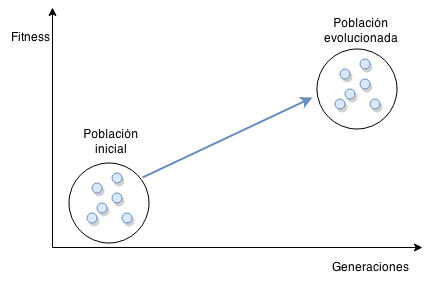
\includegraphics[width=8cm]{Figures/fitness_generaciones}
	\caption{La evolución se produce al mejorar el fitness de la población a lo largo de las generaciones.}
	\label{fig:fitness_generaciones}
\end{figure}



Por tanto se van seleccionando, combinando y cambiando las mejores soluciones en un proceso que va obteniendo mejores soluciones.
El criterio de parada nos indica cuando termina este proceso, ya sea por que se alcanzó un número de generaciones predefinidos o por que la mejora no es evidente. Al final se devuelve la mejor solución encontrada en todo el proceso.

Hay que indicar que no es una técnica exacta pero logra muy buenas aproximaciones, ademas es muy buena en problemas complejos por su flexibilidad y robustez. 


\subsubsection{Representación de soluciones}
No podemos trabajar directamente sobre las soluciones, por lo que tenemos que codificarlas en un modelo que nos sirva para poder aplicar el algoritmo.
La inspiración biológica se ve en los nombres que adopta esta representación, llamada Cromosoma que es un vector de genes y cada valor de un gen se llama alelo.
En general se codifica un vector de números binarios o reales de largo fijo, lo que facilita la aplicación de los operadores.

\begin{figure}[H]
	\centering
	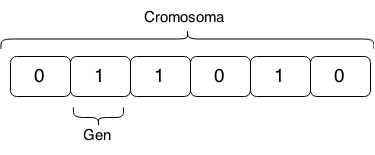
\includegraphics[width=8cm]{Figures/rep_binaria}
	\caption{Representación binaria de un cromosoma.}
	\label{fig:rep_binaria}
\end{figure}


\subsubsection{Función de Evaluación} 
Indica que tan bueno es un individuo para resolver el problema en cuestión con un valor conocido como Fitness. Este se utiliza para seleccionar a los mejores y de esta forma guiar la exploración hacia la mejor solución.
Se deben tener en cuenta las restricciones del problema para que las soluciones no factibles no sobrevivan.
En general es donde se consume el mayor tiempo del algoritmo en comparación con los demás operadores.

\subsubsection{Operador de Selección}
Existen diversos operadores de selección , su función es que las mejores características de los individuos se mantengan en las siguientes generaciones.
Los tipos más populares son:

\begin{itemize}
	\item Ruleta: También conocida como selección proporcional elige aleatoriamente individuos en la cual la probabilidad de selección es proporcional al valor de fitness.
	\item Torneo: Se elige aleatoriamente un determinado número de individuos los cuales compiten entre si usando su valor de fitness.
	\item Rango: Se ordenan los individuos por fitness y se seleccionan los mejores.
\end{itemize}

\subsubsection{Cruzamiento}
Su función es combinar individuos con el objetivo de preservar las mejores características y así lograr mejores soluciones. 
Existe una tasa que se puede modificar para indicar la probabilidad de que se realice el cruzamiento.

\begin{itemize}
	\item Cruzamiento de un punto: A partir de dos padres se selecciona un punto al azar de los cromosomas obteniendo dos trozos que se combinan para obtener dos hijos. Se explica en la figura ~\ref{fig:cruzamiento1}
	\item Cruzamiento multipunto: El método anterior se puede generalizar para obtener más puntos de corte y más recombinaciones.
\end{itemize}

\begin{figure}[h]
	\centering
	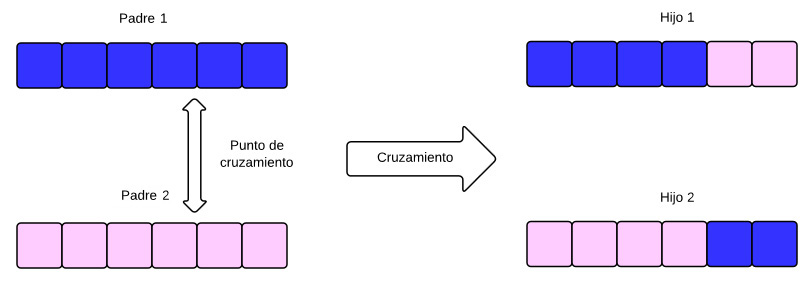
\includegraphics[width=\textwidth]{Figures/cruzamiento1}
	\caption{Cruzamiento de un punto}
	\label{fig:cruzamiento1}
\end{figure}

\subsubsection{Mutación} 
Indica el método utilizado para modificar un individuo, esto se realiza para lograr más diversidad y no caer en máximos locales. En general aplica una modificación aleatoria en el cromosoma.Hay una tasa de probabilidad para aplicar este operador que en general es muy baja. 
\begin{figure}[h]
	\centering
	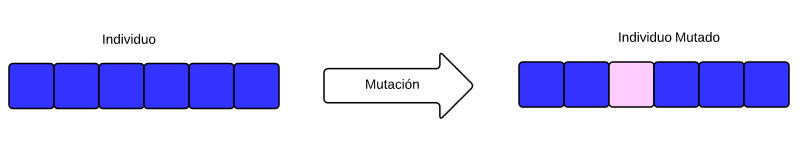
\includegraphics[width=1\linewidth]{Figures/mutacion1}
	\caption{Mutacion por inversión binaria}
	\label{fig:mutacion1}
\end{figure}


\subsubsection{Reemplazo} 
Luego de que se aplica el cruzamiento se insertan nuevos individuos que aumentan la población original por tanto este operador indica cual es el criterio que debemos tomar para crear una nueva población con una cantidad de individuos igual a la original.
Se podría reemplazar todos los padres por los hijos, o seleccionar cuales reemplazar, entre otros criterios.

\subsubsection{Criterio de parada} 
Indica cuando debe terminar el algoritmo, puede ser definiendo un número fijo de generaciones o analizando si el mejor valor de fitness se mantiene relativamente constante durante un número determinado de generaciones entre otros criterios. El objetivo sera encontrar un compromiso entre un buen resultado y un tiempo acorde de ejecución, ya que el algoritmo no arrojara un valor exacto sino una buena aproximación. 

\subsection{Funcionamiento}

El esquema básico de funcionamiento es el siguiente:


\begin{algorithm}%[!ht]
	\caption{Algoritmo Genético}
	\label{alg:algoritmo_genetico_simple}
	\begin{algorithmic} [1] 
		{
			%\small
			\STATE {Inicializo( Pob(0))}
			\STATE \texttt{generacion} = 0
			\WHILE {\text{No llegue al criterio de parada}}
			\STATE {Evaluar Pob(generacion)}
			\STATE {Padres = Seleccionar(Pob(generacion))}
			\STATE {Hijos = Cruzamiento(Padres) y Mutacion(Padres)}
			\STATE {NuevaPob = Reemplazar Pob(generacion) con Hijos}
			\STATE \texttt{generacion}++
			\ENDWHILE
			\RETURN Mejor solución
		}
	\end{algorithmic}
\end{algorithm}



% ctrl+t comenta
%\begin{algorithm}%[!ht]
%	\caption{Genetic Algorithm}
%
%	\begin{algorithmic} [1] 
%		{
%
%			\STATE {Init( Pop(0))}
%			\STATE \texttt{generation} = 0
%			\WHILE {\text{NOT Stop Criteria}}
%			\STATE {Evaluate Pop(generation)}
%			\STATE {Parents = Selection(Pop(generation))}
%			\STATE {Children = Crossover(Parents) and Mutation(Parents)}
%			\STATE {NewPop = Replace Pop(generation) with Children}
%			\STATE \texttt{generation}++
%			\ENDWHILE
%			\RETURN Best solution
%		}
%	\end{algorithmic}
%\end{algorithm}


\subsection{Algoritmos genético multiobjetivo}

Los problemas de optimización multiobjetivo trabajan sobre un espacio multidemensional de funciones y no tienen una única solución por esto el significado de optimo cambia. Una solución es un optimo de Pareto si ninguna de las funciones objetivos puede mejorar su valor sin degradar otro de los valores objetivos. Todas las soluciones de Pareto son consideras igualmente buenas ya que los vectores no se pueden ordenar completamente. Al conjunto de los valores funcionales de los optimos de Pareto se les llama frente de Pareto.

Existen algoritmos evolutivos para resolver el problema de la optimización multiobjetivo estos son los llamados MOEA por sus siglas en ingles \emph{ MultiObjetive Evolutionary Algorithm}. Para un análisis mas detallado se recomienda el trabajo de \citet{Deb2001}.

Lo que buscan es aproximarse al frente de Pareto y lograr mostrar una gama de diferentes compromisos entre las funciones a optimizar para luego poder tomar la decicion de cual elegir.


\begin{algorithm}%[!ht]
	\caption{Algoritmo Evolutivo MultiObjetivo. En rojo se indican las diferencias con el algoritmo evolutivo genérico.}
	\label{alg:algoritmo_genetico_multiobjetivo}
	\begin{algorithmic} [1] 
		{
			%\small
			\STATE {Inicializo( Pob(0))}
			\STATE \texttt{generacion} = 0
			\WHILE {\text{No llegue al criterio de parada}}
			\STATE {Evaluar Pob(generacion)}
			\STATE {\textcolor{red}{Operador Diversidad (Pob(generacion))}}
			\STATE {\textcolor{red}{Asignar Fitness (Pob(generacion))}}
			\STATE {Padres = Seleccionar(Pob(generacion))}
			\STATE {Hijos = Cruzamiento(Padres) y Mutacion(Padres)}
			\STATE {NuevaPob = Reemplazar Pob(generacion) con Hijos}
			\STATE \texttt{generacion}++
			\ENDWHILE
			\RETURN 	{\textcolor{red}{Frente de Pareto}}
		}
	\end{algorithmic}
\end{algorithm}

Hay dos operadores propios de los MOEA estos son el operador de diversidad y el operador de asignación de fitness. El primero se aplica para evitar la convergencia a un sector en particular del frente de Pareto, el segundo intenta brindar mayor chance de perpetuar a los individuos con mejores características.

Se pueden clasificar por el método de asignación de fitness en:
\begin{itemize}
	\item No basado en Pareto: Utilizan métodos sencillos de asignación de fitness. Son adecuados cuando el problema tiene no mas de tres funciones objetivo. Un mecanismo popular es la combinación lineal de los objetivos.
	\item Basado en Pareto: Utiliza explícitamente la dominancia de Pareto al asignar el fitness.
\end{itemize}



\subsection{Algoritmo Evolutivo Paralelo}
Los problemas complejos suelen requerir una alta demanda computacional por lo que paralelizar el algoritmo evolutivo es útil para lograr tiempos de ejecución menores, pero no es el único objetivo que se puede conseguir, entre otros tenemos:  encontrar soluciones alternativas al mismo problema, búsqueda mas eficiente aun sin hardware paralelo, facilidad en la cooperación con otros métodos de búsqueda y búsqueda paralela de múltiples puntos en el espacio. \citep{Alba2002}. 


Existen varios niveles de paralelización ya sea a nivel global enfocándonos en paralizar la función fitness, a nivel de la población, o a nivel del individuo. \citep{Nesmachnow2002}

En el caso de los algoritmos genéticos gran parte del tiempo se ocupa en la etapa de evaluación, por esta razón es un buen método para distribuir la carga en varios procesadores para que las evaluaciones se realicen en paralelo. 

Un modelo muy utilizado es el Maestro-Esclavo. El proceso maestro es el encargado de realizar los operadores básicos del algoritmo y distribuir a procesos esclavos la evaluación de la función fitness para un conjunto de individuos, el esclavo devuelven el resultado y luego el maestro es el encargado de continuar ejecutando los operadores.

De este modo aumenta la eficiencia computacional del algoritmo ya que una de las funciones más costosas es distribuida entre varios nodos.

\begin{figure}[H]
	\centering
	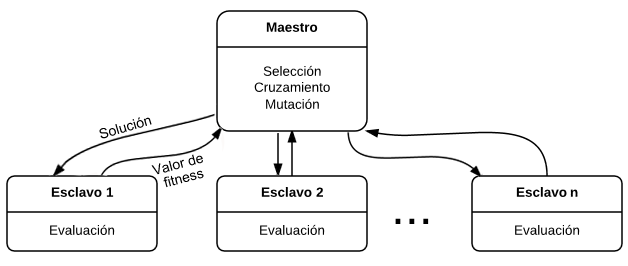
\includegraphics[width=0.7\linewidth]{Figures/diagrama-master-slave}
	\caption[Modelo Maestro-Esclavo]{Modelo Maestro-Esclavo}
	\label{fig:diagrama-master-slave}
\end{figure}

\subsection{Resumen}
Los algoritmos evolutivos han demostrado su eficiencia en la resolución de gran cantidad de problemas de optimización.  Si nos enfocamos en el problema de la sincronización de semáforos existen herramientas utilizadas para su resolución, entre las que se encuentra los simuladores de tráfico los cuales serán explicados en la siguiente sección.


\section{Simuladores de tráfico}

Los simuladores de tráfico son programas que simulan el movimiento de vehículos sobre una red de calles. Son usados en la investigación de tráfico vehicular, estudio de congestiones y análisis de impacto de obras.  Existen varias razones para optar por esta herramienta, como es la rapidez en la obtención de resultados ya que la simulación se puede realizar en tiempos mucho más rápidos que en la realidad, el costo pues no es necesario cambiar la infraestructura para probar nuevos escenarios y sirve para prever situaciones que podrían darse bajo determinadas circunstancias.

Los simuladores se pueden dividir en microscópicos o macroscópicos según el nivel de detalle de la simulación. Un simulador macroscópico modela  el tráfico vehicular como un fluido. En cambio un simulador microscópico simula el movimiento de cada vehículo según sus características particulares.

Cuanto más crece el número de vehículos y la complejidad de la red de mapas más difícil se hace crear la entrada que necesita el simulador. Aunque existen diversas herramientas que ayudan a este proceso aún se requiere un trabajo manual para el acondicionado de estos archivos.

\citet{SUMO} es uno de los simuladores abiertos más populares. Es microscópico y utiliza una serie de archivos de configuración para representar las rutas, los vehículos y el tráfico.  


\section{Trabajos relacionados}

La investigación del estado del arte se realizo con dos objetivos en mente, el primero analizar las distintas soluciones que existen actualmente para el problema y segundo encontrar nuevas prácticas, algoritmos o utilidades que pudieran fortalecer la solución.

El problema del tráfico optimizando las luces de los semáforos se puede resolver por diferentes métodos como  redes neuronales \citep{Lopez1999}, lógica difusa \citep{Lim2001}, redes de petri \citep{DiFebbraro2002}, etc; por lo tanto la cantidad de soluciones encontradas fue abundante y variada, por esto se decidió enfocarse en soluciones cercanas a la propuesta y en otras que tuvieran alguna particularidad interesante para destacar.


\begin{itemize}
	\begin{item}
		\bibentry{Sanchez2004}
		
		Este trabajo se basa en tres puntos: El uso de algoritmos genéticos para la optimización, simulación de autómatas celulares para la función de evaluación del tráfico y un cluster para realizar ejecuciones en paralelo.
		El modelo es pequeño con 5 calles de 2 vías que se intersectan.
		La codificación del cromosoma es un vector de números enteros, donde se codifica para cada intersección cual calle está habilitada en cada ciclo.
		Usa una estrategia de selección elitista donde los dos mejores se clonan a la siguiente generación y el resto es generado por cruzamiento de dos puntos.
		
		Para la evaluación se utiliza el tiempo que transcurre desde el momento que un vehículo entra en la red hasta que sale. Se utilizo un cluster y programación paralela con una estrategia maestro-esclavo, el maestro envía los cromosomas a los esclavos que evalúan y devuelven el resultado, luego el maestro se encarga de generar la siguiente población.
		
		Se compararon los resultados con una simulación aleatoria y con una fija, obteniendo la solución propuesta mejores resultados en todos los casos evaluados.
		
		Este mismo grupo realizo trabajos similares expandiendo esta investigación, que se presentan a continuación.
	\end{item}
	
	\begin{item}
		\bibentry{Sanchez2008}
		Lo interesante de este estudio es que se aplica lo expuesto en el trabajo anterior a un lugar real en Santa Cruz de Tenerife para validar los resultados.
		Algunas mejoras que se introdujeron fueron que el cromosoma se codifica utilizando código Gray lo que dicen mejora el rendimiento en mutación y cruzamiento. La población inicial esta compuesta por nueve "soluciones" provistas por la alcaldía de la ciudad. Tanto la estrategia de selección como de cruzamiento y mutación es similar al anterior trabajo.
		
		El modelo se discretizó en 42 semáforos, 26 entradas y 20 salidas.
		Las soluciones provistas por la alcaldía se simularon y se utilizo para comparar con los resultados obtenidos por el algoritmo que en términos generales logra una mejora de hasta 26\%.
		
	\end{item}
	
	\begin{item}
		\bibentry{Sanchez2010}
		Este trabajo es similar al anterior pero se destacan algunos cambios, por ejemplo se probaron cuatro funciones de fitness diferentes, ellas fueron: cantidad de vehículos que llegaron a destino, tiempo de viaje promedio, tiempo de ocupación promedio y velocidad promedio global.
		También agrega medidas correspondientes al gas total emitido por los vehículos que tiene relación con la velocidad a la que van.
		El modelo discretizado de la zona de "La Almozara" cuenta con 17 semáforos, 7 intersecciones, 16 entradas y 18 salidas.
		Se simuló tanto un caso estándar como casos de alta congestión de tráfico, las comparaciones se hacen respecto a las distintas funciones de fitness y los distintos escenarios planteados logrando buenos resultados.
		
	\end{item}
	
	
	\begin{item}
		\bibentry{Penner2002}
		Este trabajo se centra en un modelo de simulación basado en enjambres que luego se optimiza utilizando un algoritmo genético cuya función de fitness es el tiempo promedio de los vehículos dentro de la red. El cromosoma cuenta con la secuencia y duración de los semáforos, así como la relación con los semáforos complementarios, la mutación tiene en cuenta esto para que no ocurra en una misma intersección dos luces verdes. El cruzamiento se hace entre los distintos semáforos con una probabilidad más alta si esta en la misma intersección.
		
		El primer escenario es pequeño, cuenta con una ruta de 3 carriles y 3 intersecciones.Con diferentes variaciones logra mejoras significativas.
		
		Luego se realiza otro escenario más complejo de 28 semáforos y 9 intersecciones logrando mejoras de hasta 26\%.
	\end{item}	
	
	
	\begin{item}
		\bibentry{Stolfi2012}
		Este trabajo se basa en el concepto de una ciudad inteligente enfocado en la movilidad, indica que los atascos del tráfico provocan tanto perdidas económicas como también contaminación ambiental.
		
		Utiliza un algoritmo inteligente que tomando en cuenta el estado de congestión de las rutas sugiere al usuario cual es la ruta más rápida a su destino, utilizando un dispositivo en el automóvil que se enlazara por wifi con los semáforos que cuentan con sensores. Por lo tanto el trabajo no se basa en la optimización de las señales de los semáforos existentes sino agrega encima de esto un sistema de búsqueda de mejor ruta.
		
		Para el modelo utiliza una zona  de la ciudad de Málaga, cuenta con 8 entradas y 8 salidas, para la simulación utiliza \citet{SUMO}. Los vehículos modelados son: turismo, monovolumen, furgoneta y camión donde se varia la longitud, velocidad y probabilidad que entre en la red de tráfico.
		
		Se intenta minimizar los tiempo de viaje de los vehículos que circulan por la red. Para ellos se utiliza un algoritmo genético cuya estrategia de selección consiste en tomar los dos peores individuos reemplazándolos por los dos mejores hijos encontrados. En el cromosoma se representa cada sensor, con los destinos y rutas posibles. La función de fitness tiene en cuenta la cantidad de viajes completados durante el tiempo de ejecución, el tiempo medio utilizado y el retraso medio. Se prueban varias estrategias de cruzamiento y mutación. Las ejecuciones tienen un tiempo fijo de duración.
		
		
		Compara el resultado con una simulación donde se generaron 64 itinerarios diferentes, esto se prueba en 3 escenarios. Las simulaciones se realiza hasta con 800 vehículos, concluyendo que al aumentar la cantidad de vehículos (más de 400) en el sistema la solución mejora sustancialmente el resultado base.
		
	\end{item}	
	
	
	\begin{item}
		\bibentry{Teo2010}
		Este trabajo presenta un modelo simple con una sola intersección en donde se intenta optimizar los tiempos de los semáforos para lograr mejorar rendimiento del trafico. El cromosoma representa los tiempos de la luces verdes mientras que la función de fitness es el largo de las colas generadas. Un aspecto interesante es que la simulación tiene un tiempo fijo de 600 segundos por generación pero no se detalla el tipo de simulación utilizada. Las conclusiones indican que la optimización usando algoritmos genéticos  es buena para el problema del flujo de tráfico.	
	\end{item}	
	
	
	\begin{item}
		\bibentry{Montana1996}
		Esta propuesta utiliza un enfoque adaptativo con sensores que analizan el tráfico en tiempo real. Un sensor para saber cuantos autos pasan y otro para saber que tan larga es la cola. Considera los cambios que se producen con respecto al caso promedio y cambia los tiempos de las señales en forma acorde.
		La premisa se basa en la inteligencia colectiva en donde agentes individuales realizan tareas simples que al interactuar producen resultados globales.
		
		Se aplica programación genética más específicamente STGP (strongly typed genetic programming) \citep{Montana1995} que aprende el árbol de decisión que sera ejecutado por todas las intersecciones cuando decida el cambio de fase. Además un algoritmo genético híbrido busca diferentes constantes que serán usadas en los arboles de decisión mejorando el flujo de tráfico.
		
		La medida básica de efectividad en la función de evaluación es el \emph{Delay}, esto es el total de tiempo perdido por causa de las señales de tráfico. Se probaron tres modelos distintos de cuatro intersecciones con una versión especial del simulador  TRAF-NETSIM \citep{TRAF-NETSIM}
		
		El experimento arroja buenos resultados en cuando a la performance de la red y destaca la buena adaptabilidad en diferentes circunstancias. Aunque se marca el hecho de que el modelo es simple y de tamaño pequeño, siendo una incógnita como funcionara con problemas más complejos.
		
	\end{item}	
	
	
	\begin{item}
		\bibentry{Vogel2000}
		
		La solución utiliza un enfoque auto-adaptable para mejorar el tráfico tanto en el corto como en el largo plazo a través de la optimización de las señales de tráfico en las intersecciones de una red de rutas. Al darle dinamismo a cada intersección se mejora el rendimiento de la red.
		
		Destaca el hecho que dada una configuración de semáforos aún siendo optimizada usando simulaciones es difícil que sea la mejor en todas las situaciones o en casos extremos (horas picos). Para solucionar esto proponen un sistema auto-adaptable que toma la información del tráfico actual usando detectores de vehículos y espacios.
		
		Utiliza el concepto de fases para representar las distintas posibilidades en la señalización de la intersección y cuanto tiempo debe permanecer en esa fase. 
		Propone el desarrollo de un algoritmo evolutivo donde cada individuo representa un sistema de fases mientras el fitness se obtiene simulando ese sistema en un modelo de tráfico. Este es relativamente pequeño con una intersección con cuatro brazos, cada uno con tres lineas donde la ruta principal tiene el doble de densidad vehicular. 
		
		Los resultados indican que la ventaja de usar conocimiento experto para configurar los parámetros iniciales es mínimo ya que llega muy rápido a resultados similares. Tanto la búsqueda de los mejores parámetros como en estructuras más simples el algoritmo se comporta con buenos resultados.
		
	\end{item}	
	
	\begin{item}
		\bibentry{Rouphail2000}
		
		Se estudia una pequeña red de tráfico de nueve intersecciones con semáforos en la ciudad de Chicago, contando con trafico de vehículos, parking, rutas de ómnibus y paradas.  
		Se toman valores reales en horas pico, comprobando que las colas que se generan en la simulación coinciden con la realidad.
		Usa el programa \citep{TRANSYT-7F} que permite visualizar mapas y contiene optimización de varios algoritmos genéticos y \citep{CORSIM}  un simulador de tráfico comercial.
		Se probaron 12 estrategias distintas de resolución midiendo el tiempo de demora en la red y el largo de las colas producidas. Los resultados indican que la performance de la red aumentó considerablemente usando este método.	
	\end{item}	
	
\end{itemize}


\subsection{Resumen}
Aquí un breve repaso sobre los trabajos evaluados y su comparación con la propuesta presentada.

El trabajo de \citet{Sanchez2004} posee algunos puntos de contacto como es la ejecución paralela en un cluster y la arquitectura maestro-esclavo. La principal diferencia es que el escenario que evalúan es pequeño y no se compara con un escenario real.

El siguiente trabajo de \citet{Sanchez2008} expande lo anterior y lo utiliza en un caso real en Santa Cruz de Tenerife siendo de una complejidad similar a Garzón en términos de cantidad de cruces y semáforos. Los resultados obtenidos son muy positivos obteniendo mejoras de hasta 26\%.

Se destaca de \citet{Sanchez2010} las pruebas de diferentes funciones de fitness teniendo en cuenta diversos factores como tiempo de viaje o velocidad promedio. Este trabajo inspiro la realización de una función multiobjetivo que tuviera en cuenta la velocidad promedio en el proyecto actual.

Aunque \citet{Stolfi2012} no optimiza la configuración de los semáforos, si plantea una posibilidad interesante para mejorar el trafico en una ciudad indicando a los vehículos la mejor ruta por lo que se podría tomar como un elemento en trabajos futuros.

Tanto los trabajos de \citet{Teo2010} como \citet{Stolfi2012} plantean la simulación con un tiempo fijo lo que se utilizó en el proyecto.

\citet{Montana1996} y \citet{Vogel2000}  proponen algoritmos que se adapten en tiempo real por lo que se destacan como posibles trabajos a futuro.
Es digno de mención que todos los trabajos consultados lograron mejoras significativas en sus resultados.

En conclusión el estudio de los trabajos relacionados permitió conocer en profundidad distintas soluciones y métodos que fueron tenidos en cuenta en menor o mayor medida en la solución propuesta. El hecho de que se obtuvieran buenos resultados motivo aun mas el desarrollo del trabajo presentado.





